\chapter{Experimental Setup}

We will discuss the accelerator setup used to collide gold nuclei at relativistic energies which briefly create the strongly interacting medium of quarks and gluons which we wish to study. We also examine the STAR detector, triggering, data aquisition, and its particle identification capabilities. We will specifically talk about the detector subsystems which are most relavant to the identification of electrons from heavy flavor processes. 

\section{Relativistic Heavy Ion Collider}

The Relativistic Heavy Ion Collider (RHIC) is an accelerator facility located at Brookhaven National Lab which was built for the study of QCD. The collider is capable of colliding a variety of heavy nuclei (to date: gold, uranium, and copper) as well as lighter particles (protons, deuterons, and recently helium-3). RHIC is also capable of colliding polarized proton beams for the program studying the spin structure of the proton. The top energy for collisions in RHIC is 500 GeV for p+p and 200 GeV for Au+Au. 

The main collider rings at RHIC are 2.4 miles in miles in circumference and intersect at six interaction points. Particles are brought up to collision energies through a series of linear accelerators and booster synchrotrons. Figure~\ref{fig:RHIC} shows the layout of the RHIC facilities as well as the location of the current experiments running at RHIC.

\begin{figure}[htbp]
\begin{center}
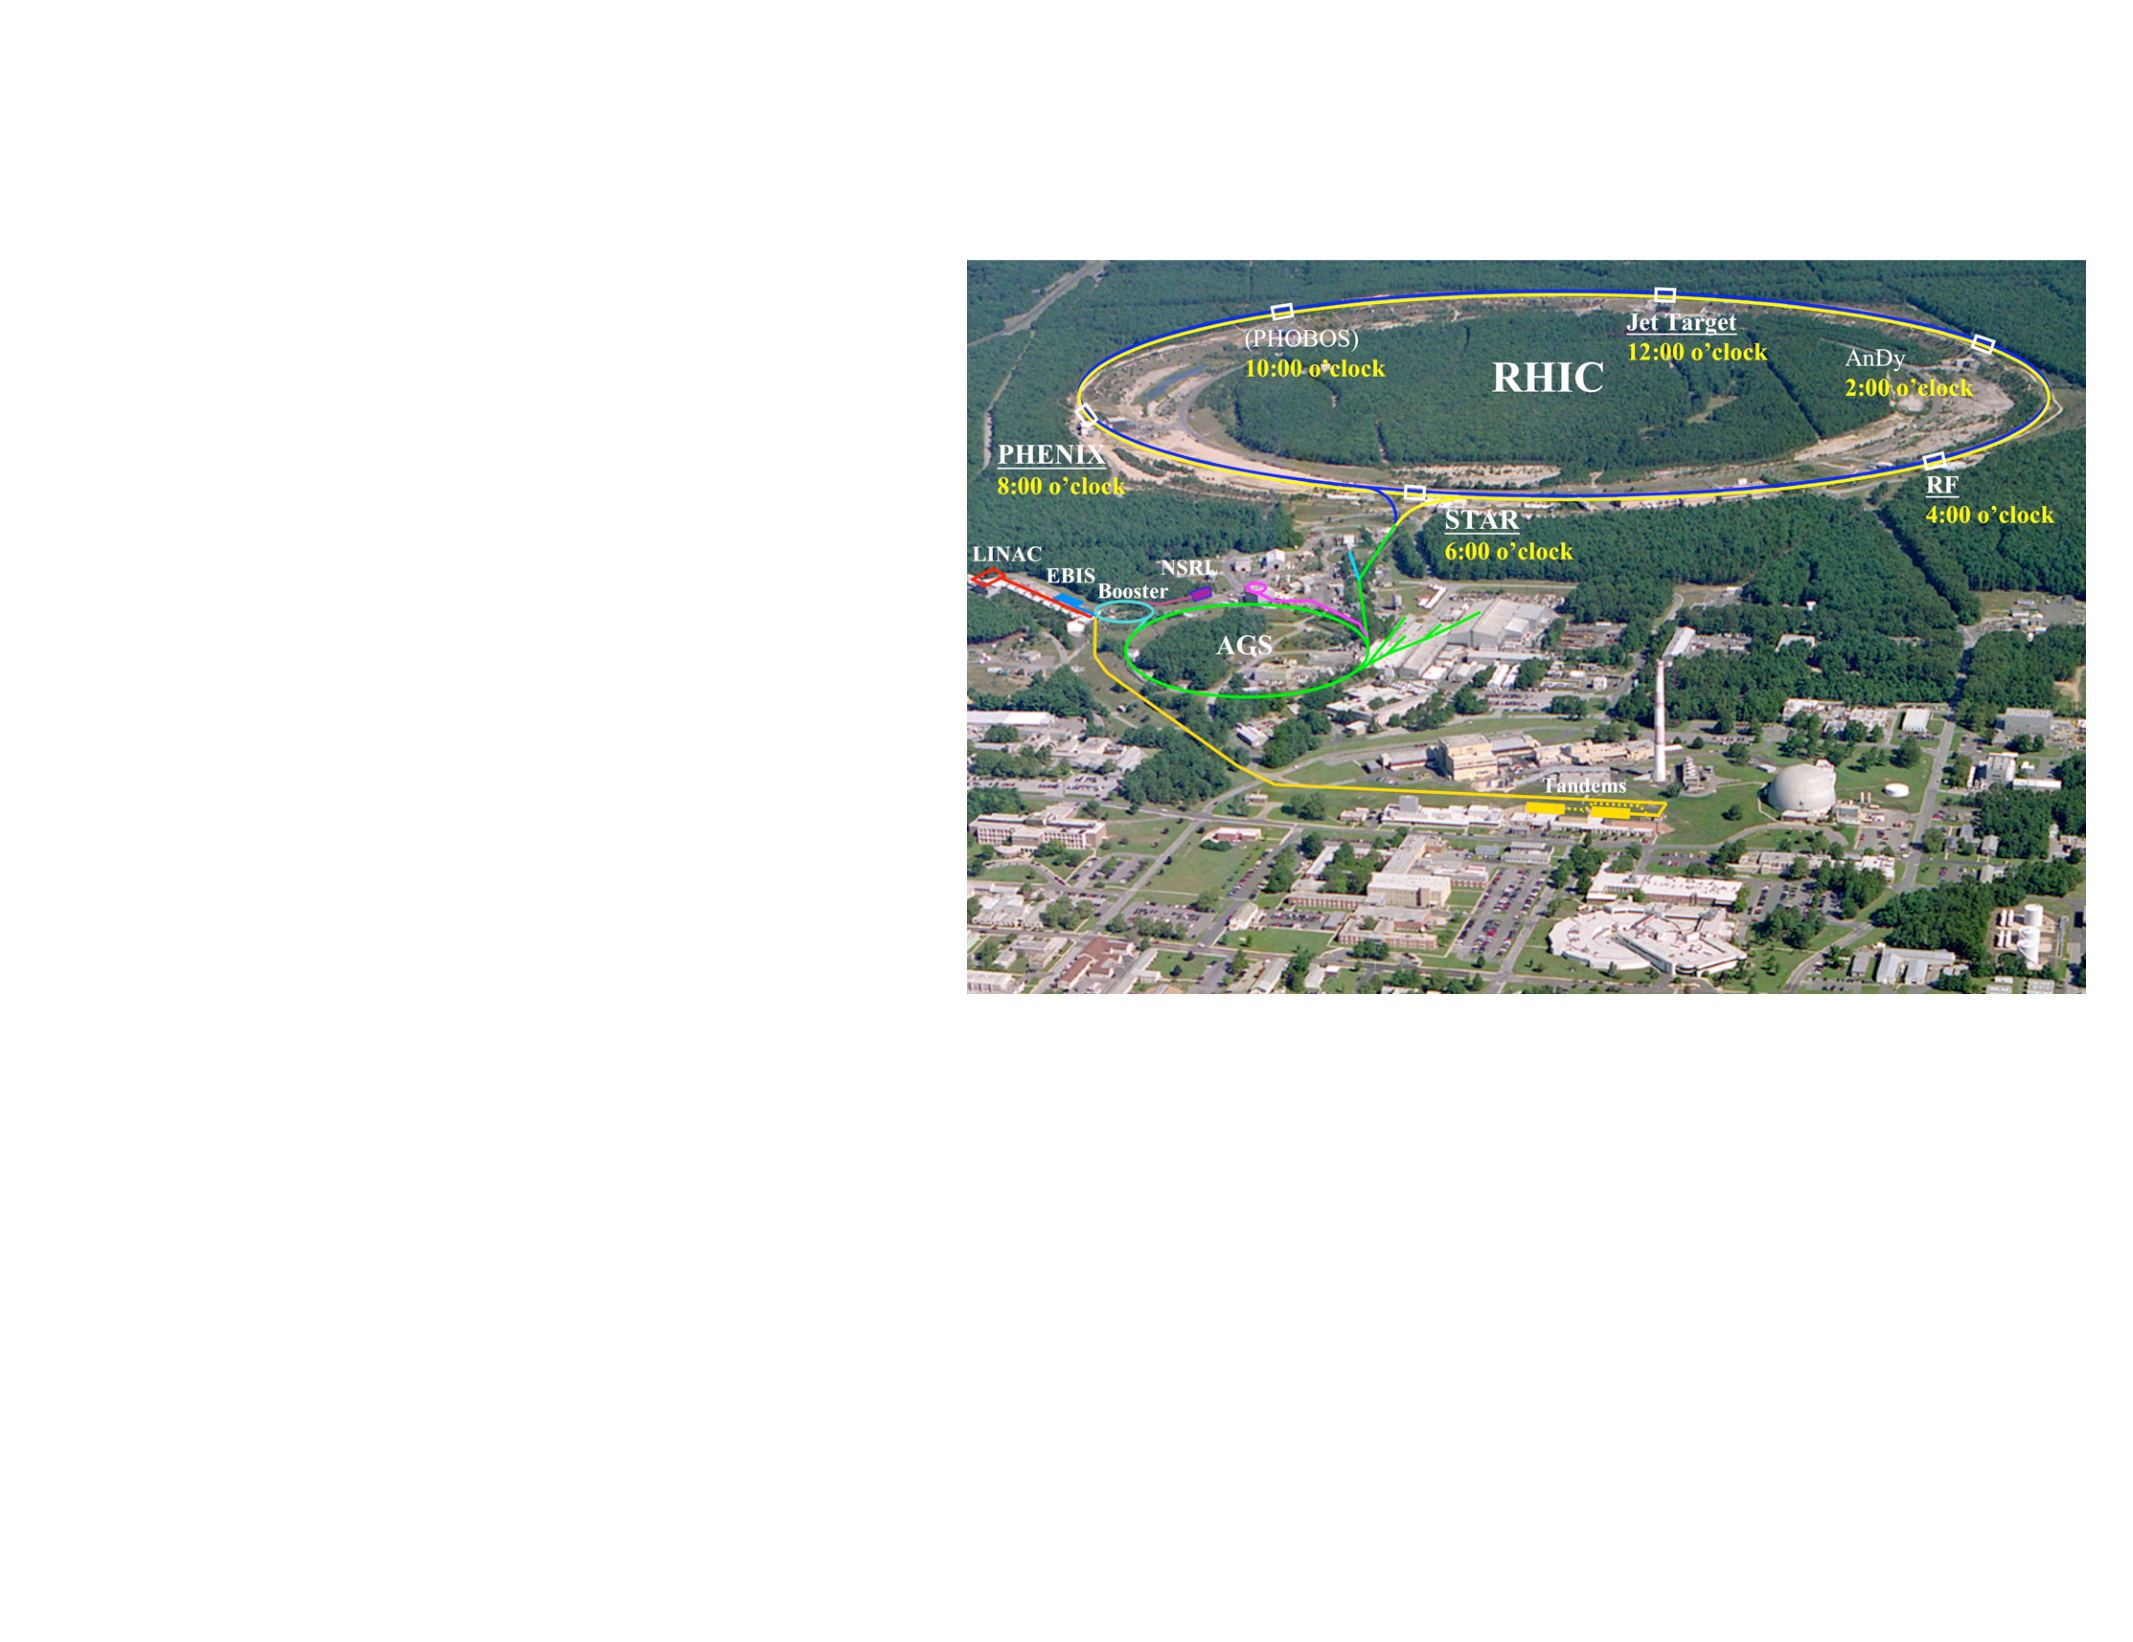
\includegraphics[scale=0.7]{Plots/Detector/RHIC_Complex.pdf}
\end{center}
\caption[RHIC Facility]{RHIC Complex seen from above. Top of the picture shows the main rings and locations of various experiments. Lower part shows the LINAC and booster rings.}
\label{fig:RHIC}
\end{figure}

For the run in 2011 gold nuclei were generated from an ion source and then initially accelerated in the Tandem Van de Graff line. RHIC had multiple Van de Graff accelerators allowing for collisions between mixed nuclei (for example, Au+Cu or d+Au). From 2012 onwards, the function of the tandems was replaced by the Electron Ion Beam Source (EBIS) which generates particles from deuterons to uranium nuclei. Protons beams on the other hand originate from the 200 MeV LINAC. Both protons and other nuclei move to the booster synchrotron which further accelerates the particles using RF waves. After passing through the booster ring the beams then enter the Alternating Gradient Synchrotron (AGS). The AGS was a long running and highly succesful facility at BNL, three Nobel Prizes resulted from research conducted at AGS. Now AGS serves as a final booster ring before sending the beams to the main RHIC rings. 

The beams then reach RHIC where the last remaining electrons are stripped away leaving only the nuclei. In the storage rings the particles circulate in bunches, typically around 110 bunches per ring, and the beams are brought to their collision energy. The beams can collide at six interaction points along the ring. Top energy for the heavy ion program in 200 GeV per nucleon, higher energies are used in some p+p collisions and RHIC is also capable of colliding at lower energies as is the case in the beam energy scan program which explores the QCD phase diagram.

\section{STAR Detector}

The Solenoidal Tracker at RHIC (STAR) is a general purpose detector located at the 6 o'clock interaction point at RHIC. STAR consists of a variety of detector subsystems which cover a large acceptance region and allow for a variety of physics programs. This analysis will focus only on data taken with STAR's mid rapidity detectors. Figure~\ref{fig:STAR} is a diagram showing the configuration of STAR. It should be noted that for the data taking for this analysis the Silicon Vertex Tracker (SVT) was removed and only its support structure remained.

\begin{figure}[htbp]
\begin{center}
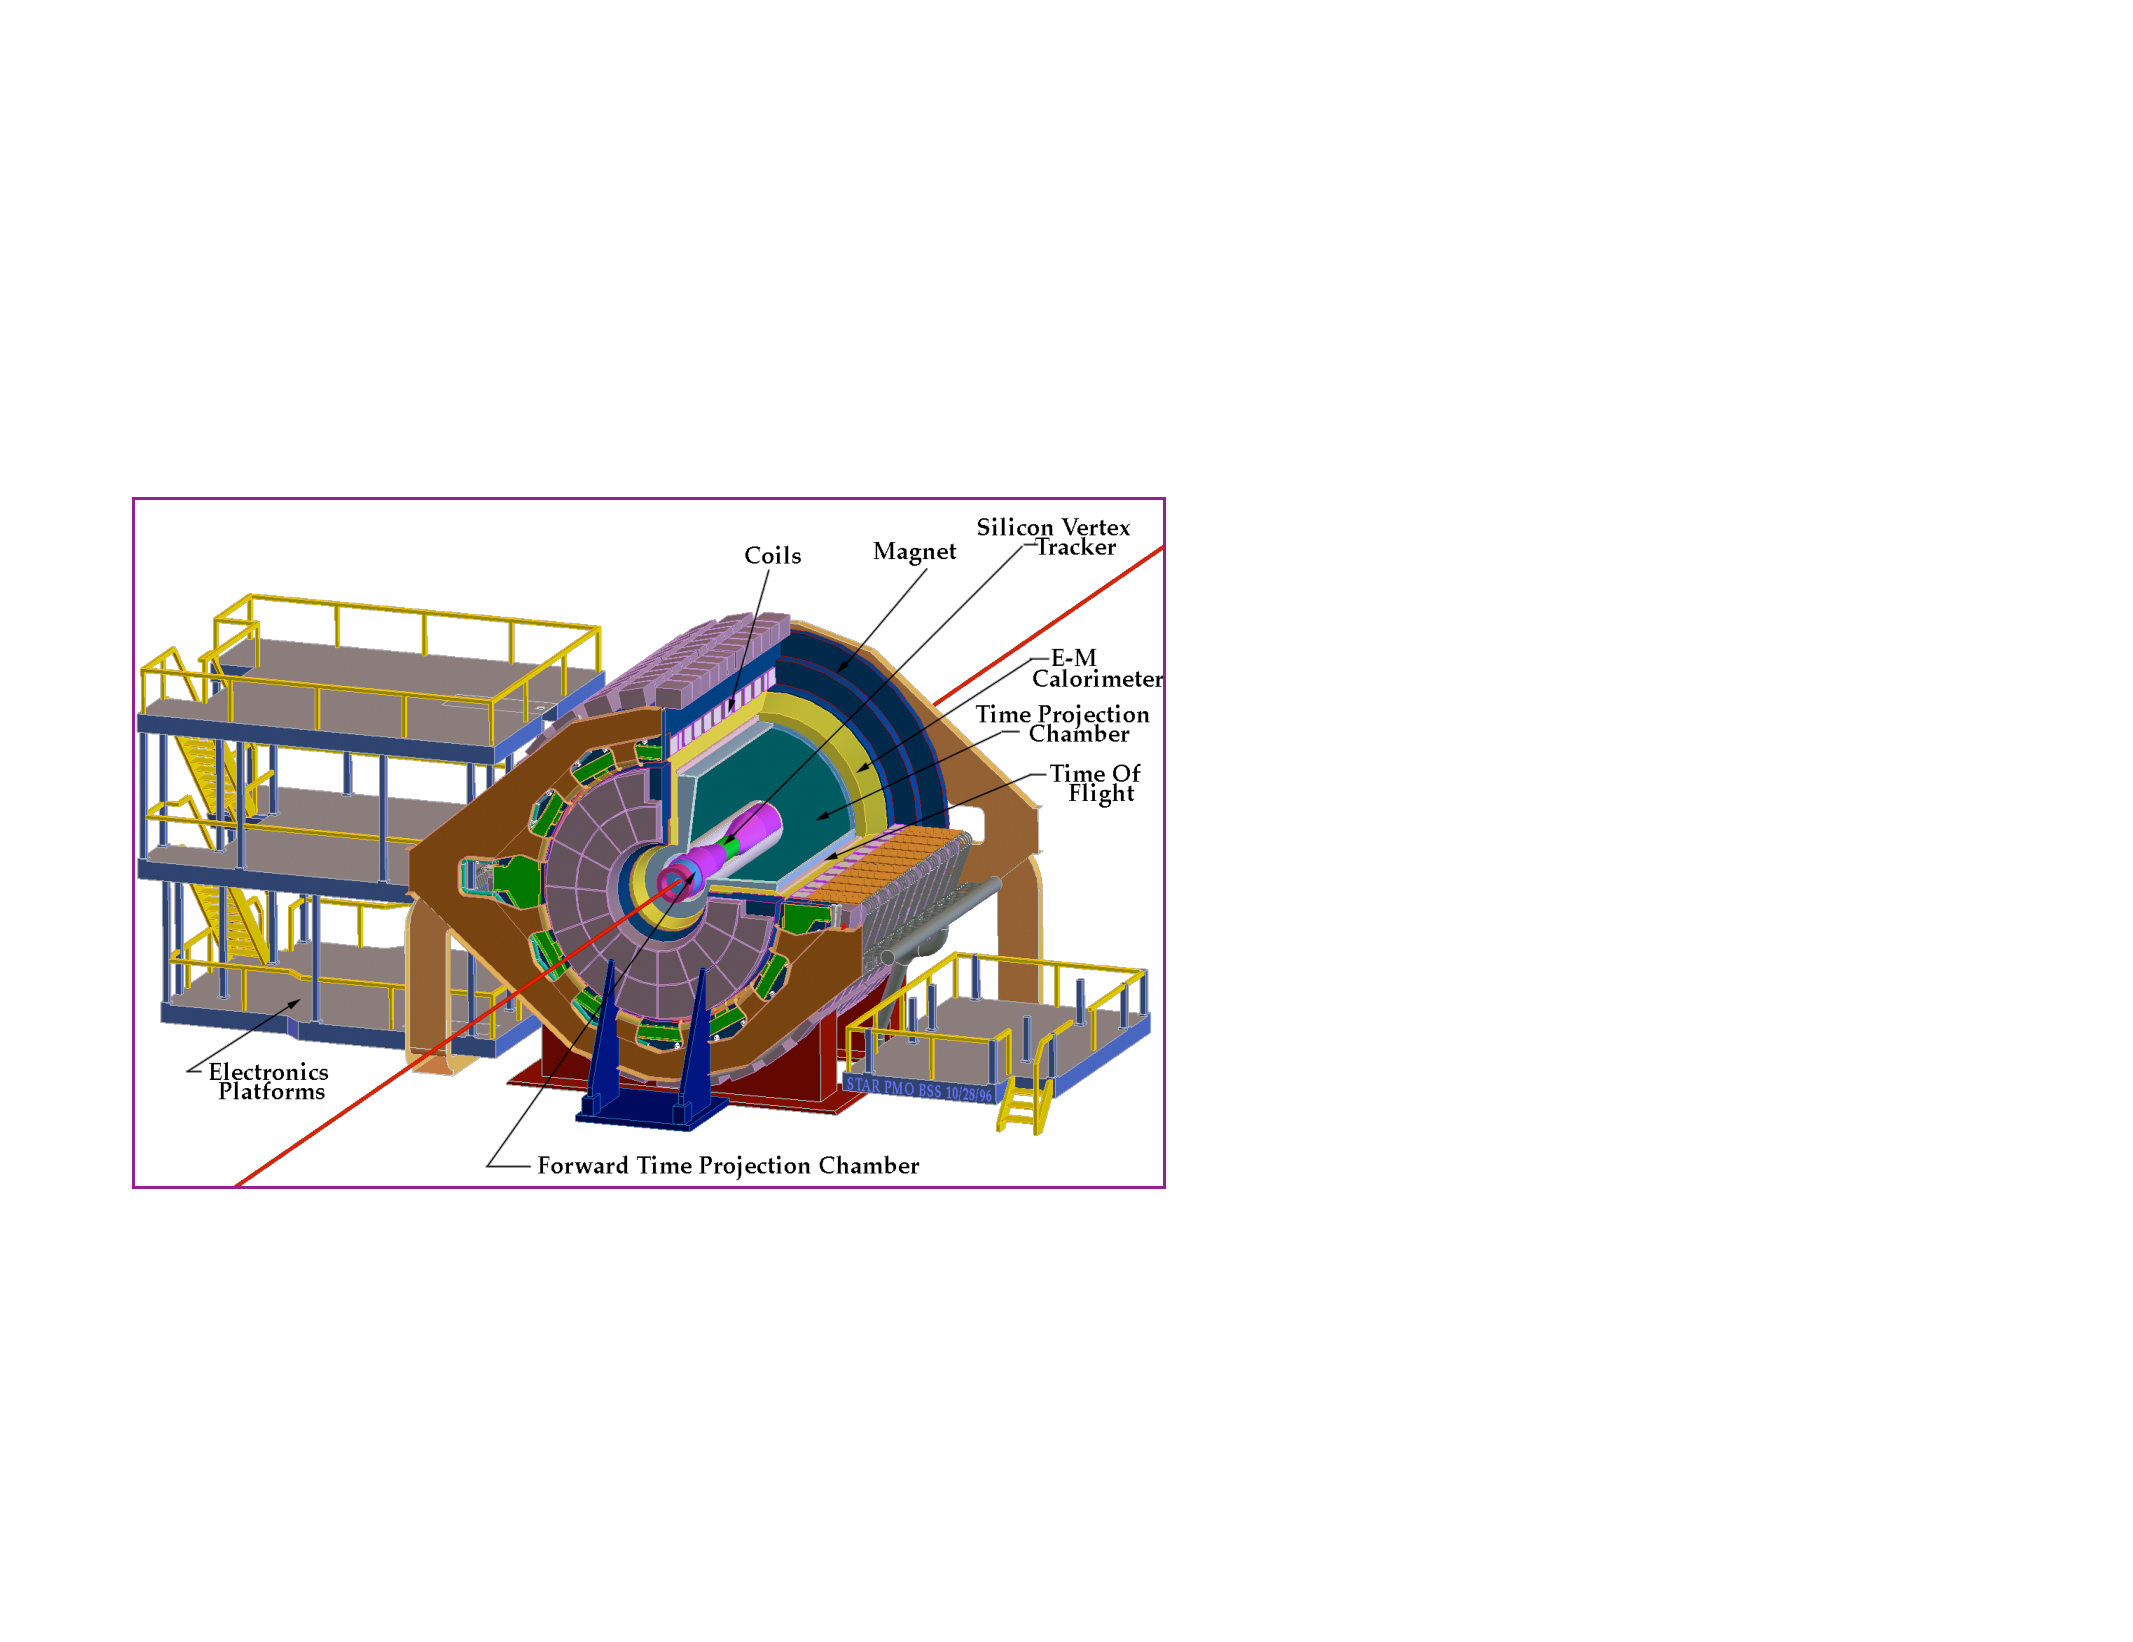
\includegraphics[scale=0.7]{Plots/Detector/STAR_Detector.pdf}
\end{center}
\caption[STAR Detector]{The STAR detector as it was configured around the time of the data taking for this analysis. The SVT was removed prior to run 10 and thus only its support structure was in during the runs.}
\label{fig:STAR}
\end{figure}

In STAR the primary tracking detector is the Time Projection Chamber (TPC) which surrounds the beam pipe, covering $2\pi$ in azimuth and capable of tracking particles in pseudorapidity up to around $\eta \approx 1.3$. The TPC is also measures ionization energy loss of charged particles, which is used for particle identification. For runs 10 and 11 the TPC was the inner most tracking detector in STAR. Prior to this the SVT was in place as a tracking detector and from 2014 onwards the inner tracking in STAR has been upgraded with the Heavy Flavor Tracker (HFT) which is capable of improving resolution on secondary vertices. Outside of the TPC is the Time of Flight (TOF) detector. TOF greatly improves the particle identification for low momentum hadrons. Further outside of TOF and the TPC is the Barrel Electromagnetic Calorimeter (BEMC): a lead-scintillator calorimeter and Shower Maximum Detector (SMD). The BEMC allows for measurements of electron energies, improves the identification of high $p_T$ electrons, and allows for identifying $\gamma$'s which cannot be tracked in the TPC. Sitting outside the BEMC is the Muon Telescope Detector (MTD) which is used for the analysis of dimuon and $e-\mu$ spectra. For measurements of non-photonic electrons we use the tracking and PID from the TPC as well as additionaly PID information from the BEMC systems.

\section{Time Projection Chamber}

The TPC is the main tracking and particle identification in STAR, it surrounds the beam pipe and interaction region and has full azimuthal coverage and covers $\pm 1.8$ in pseudorapidity. The TPC is a cylindrical volume, 4.2 m long, with an inner diameter of 1 m and an outer diameter of 4 m. The enclosed volume is filled with a mixture of 10\% methane and 90\% argon. The TPC sits inside of the STAR solenoid magnet which is capable of producing magnetic fields of .5 T in two opposite polarities. Bending of tracks of charged particles in the TPC allows for tracking of particles from .1 GeV/c to 30 GeV/c. Midway down the length of the TPC the chamber is divided by the Central Membrane. A potential is established between the Central Membrane, the cathode, and the end caps of the TPC, the anodes. Inner and Outer Field Cages run the length of the TPC along the walls, gradually increasing in potential as they get closer to the Central Membrane. The field cages help establish a uniform electric field in the TPC which is critical for tracking resolution. Figure~\ref{fig:TPC} shows an illustration of the TPC and the locations of the Central Membrane and field cages.

\begin{figure}[htbp]
\begin{center}
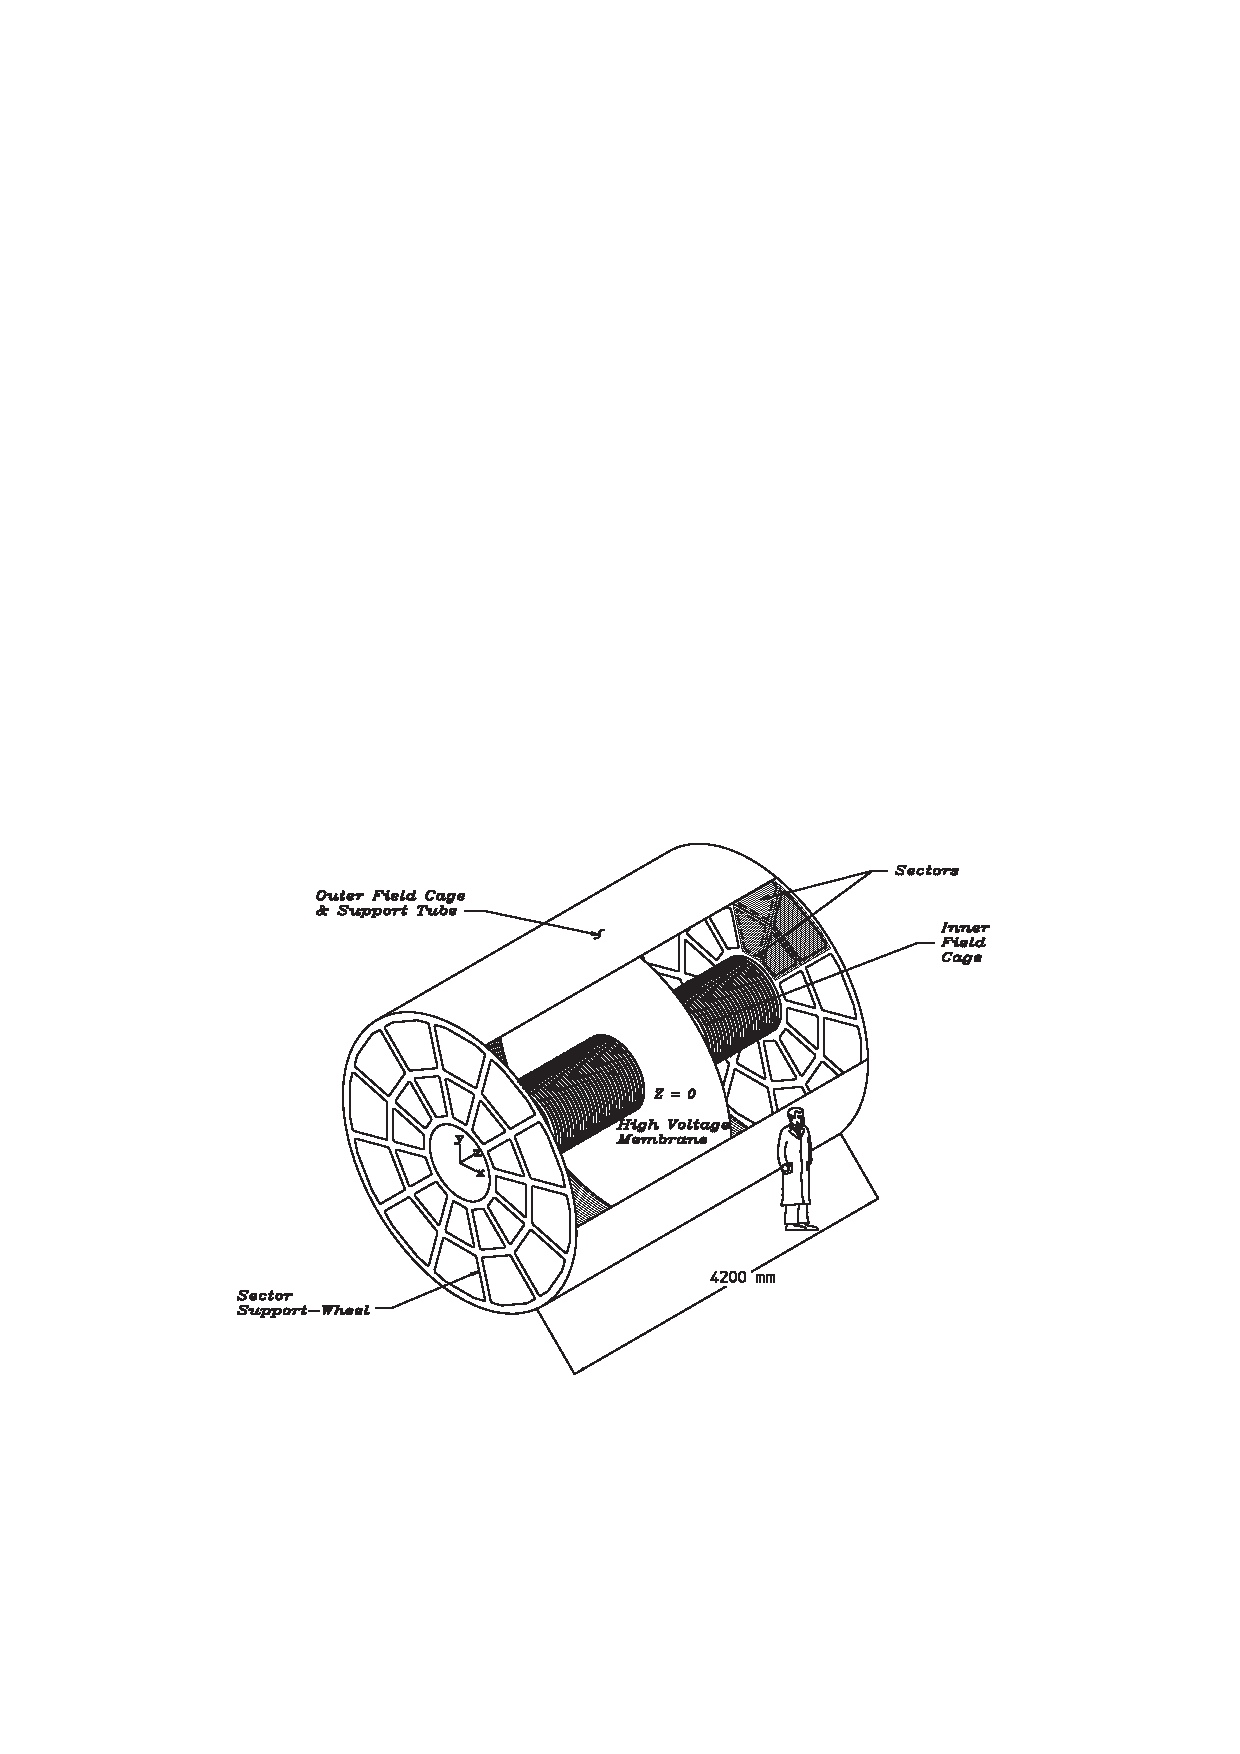
\includegraphics[scale=1.0]{Plots/Detector/TPC.pdf}
\end{center}
\caption[TPC Diagram]{Diagram of the STAR TPC showing the main components as well as the scale.}
\label{fig:TPC}
\end{figure}

Charged particles traverse the TPC and ionize the gas inside. The electrons in the drift along the electric field in the TPC at 5.45 cm/$\mu$s towards the ends of the TPC where the readout pads are located. The endcaps of the TPC chambers are divided radially into 12 sections, each section has an inner and outer segment (Figure~\ref{fig:TPC_pad}). The TPC readout sectors have 4 components, a pad plane and three wire planes. The outermost wire plane is a gating grid which can block charged particles in the TPC from reaching the readout counters at the endcap. Inside the gating grid are the ground wire plane, a readout plane and the the pad plane. The inner part of the TPC sector consists of 13 pad rows which are spaced 52 mm apart in the radial direction in the outer section there is no spacing between the pads. The inner sector also features smaller pads to improve tracking, particularly for low momentum tracks. Future upgrades to the TPC will replace the TPC sectors with ones that have no gaps between the inner pad rows. This will improve the tracking of the TPC out to larger $\eta$. 

\begin{figure}[htbp]
\begin{center}
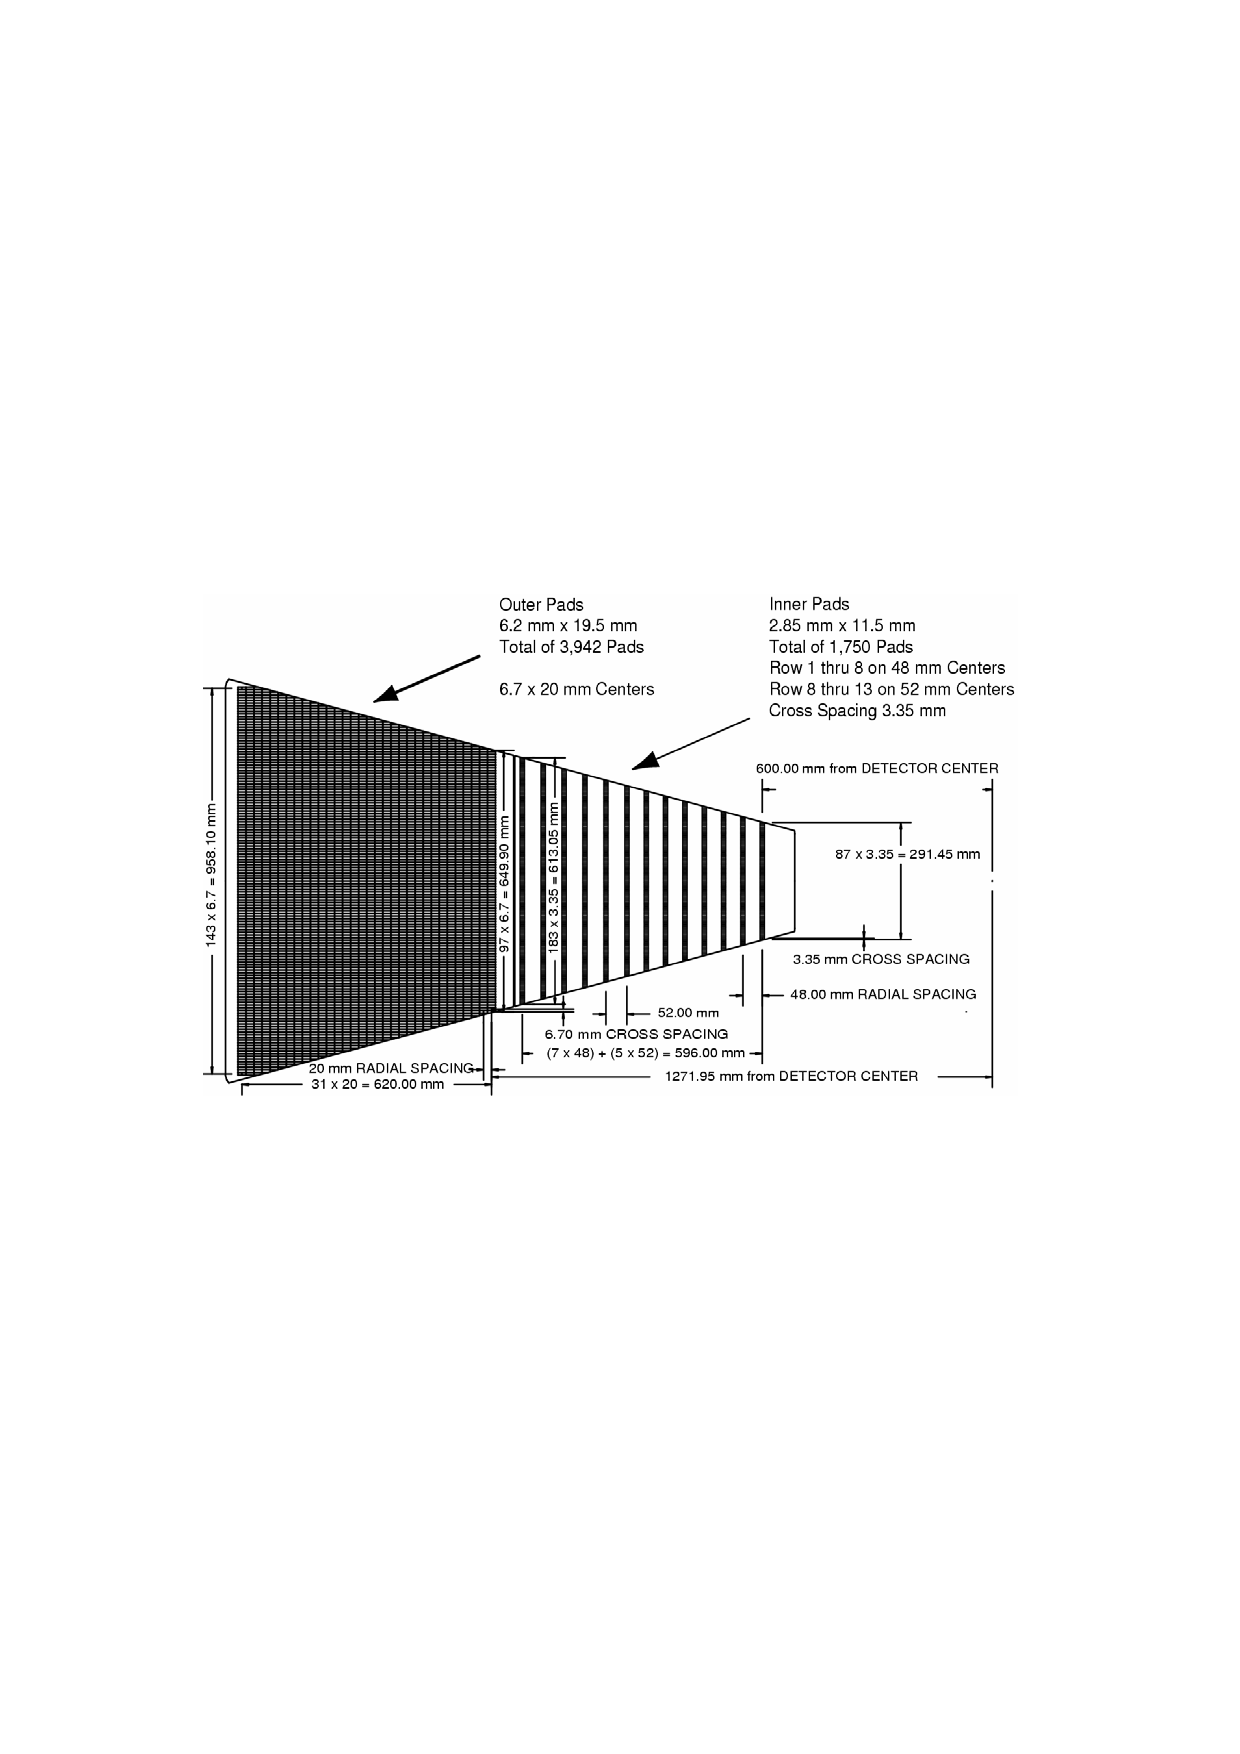
\includegraphics[scale=1.0]{Plots/Detector/TPC_pad.pdf}
\end{center}
\caption[TPC Sector]{Schematic of one TPC pad plane. The difference in spacing between inner and outer pads can be seen.}
\label{fig:TPC_pad}
\end{figure}

\section{Barrel Electromagnetic Calorimeter}

The Barrel Electromagnetic Calorimeter (BEMC) is a lead-scintillator sampling calorimeter sitting outside of the TPC and STAR magnet. The BEMC is used for studying high $\pt$ processes such as jets and (in the case of this analysis) decays from heavy mesons. The calorimeter is also used to trigger on these processes and is capable of detecting direct $\gamma$'s. There are two main subsystems of the BEMC: the towers of lead and scintillator, which produce the particle showers and collect the light to measure the energy, and the Shower Maximum Detector (SMD) for measuring the profile of showers in the BEMC which can be used to select showers from electrons.

\subsection{EMC Towers}

\subsection{Shower Maximum Detector}
